\documentclass{if-beamer}
\begin{document}
	
	\title[Campus Formoso do Araguaia]{Configuração de Redes e Servidores}
	\subtitle{Aula 2}
	\author{Gilmar Gomes do Nascimento}
	\institute[IFTO]{
		Instituto Federal do Tocantins\\
		Campus Formoso do Araguaia
	}
	\date{\today}
	\logo{
		
\includegraphics[scale=0.0085]{logo.jpg}
	}
	\subject{Servers} % metadata
	
	\graphicspath{{figuras/}}
	%---------------------------------------------------------------------------------
	\begin{frame}
		\titlepage
	\end{frame}

	\begin{frame}
		\begin{figure}
			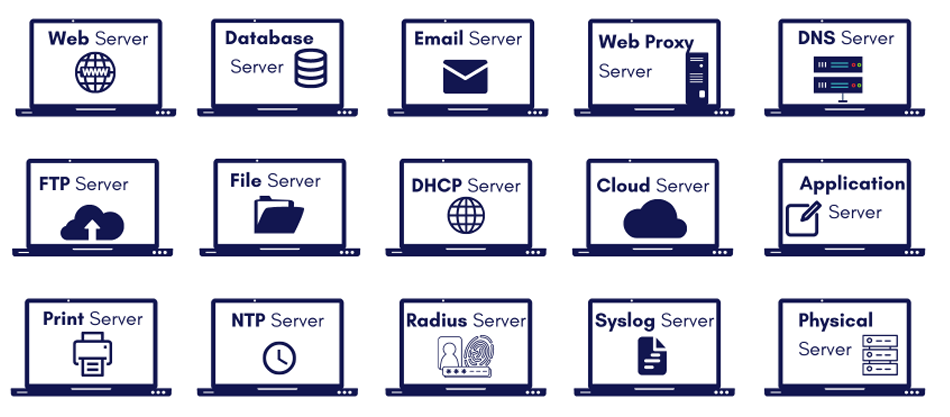
\includegraphics[scale=0.6]{servers}
		\end{figure}
	\end{frame}

	\begin{frame}{Tipos de Impressoras}
		\begin{itemize}
			\item Impressora de impacto(Matricial, margarida)
			\item Impressora de jato de tinta
			\item Impressoara a laser
			\item Impressora térmica
			\item Impressora solvente
		\end{itemize}		
	\end{frame}

	\begin{frame}{Drivers}
		\begin{figure}
			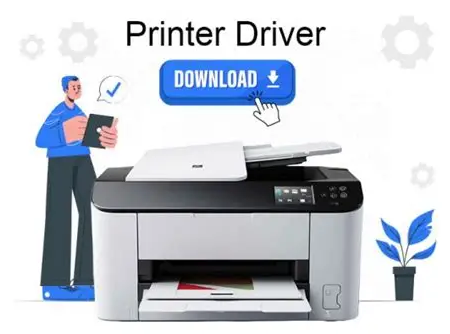
\includegraphics[scale=1]{driver-printer}
		\end{figure}		
	\end{frame}

	\begin{frame}{Terceirização de serviços}
		\textit{Outsourcing} é o termo referente à prática de negócio onde há a terceirização dos serviços relacionados
		à Tecnologia da Informação (TI). A terceirização relativa à área tecnológica consiste no processo de 
		externalização da gestão e controle de processos, além de serviços oferecidos por uma empresa privada ou governamental.		
	\end{frame}

	\begin{frame}{Guia de Boas Práticas para a Contratação do Serviço de Outsourcing de Impressão}
		\begin{figure}
			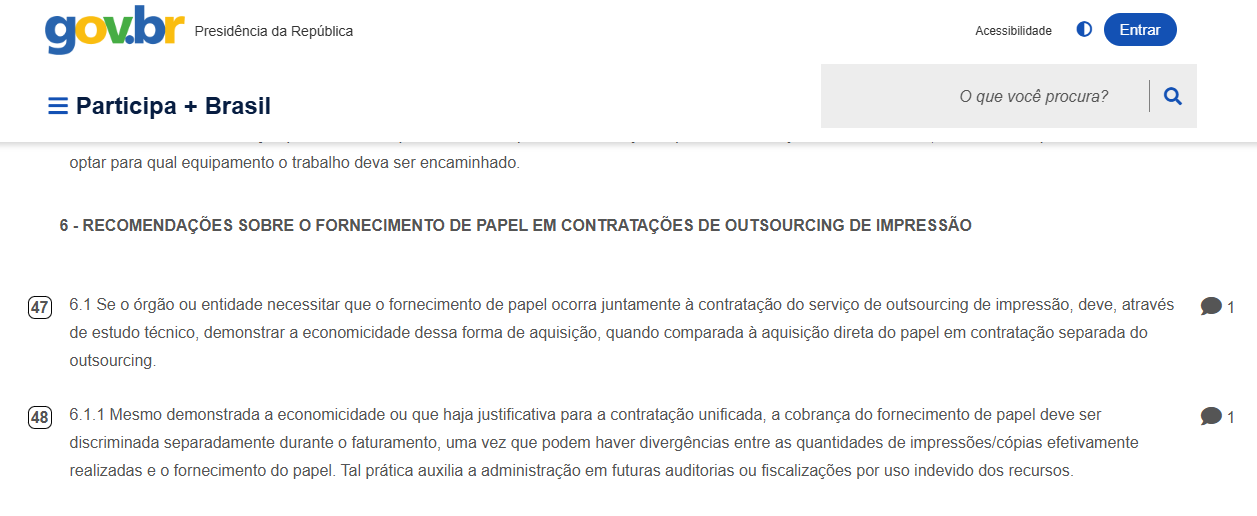
\includegraphics[scale=1]{gov-outsourcing-printing}
		\end{figure}
	\end{frame}

	\begin{frame}{Servidor de Impressão}
		\begin{itemize}
			\item MS Windows
			\item Apple
			\item GNU\Linux
		\end{itemize}		
	\end{frame}

	\begin{frame}{Impressoras e marcas}
		\begin{itemize}
			\item Xerox
			\item HP 
			\item Samsung
			\item Kyocera
		\end{itemize}
	\end{frame}

	\begin{frame}[allowframebreaks]{Kyocera Print Center}
		é um aplicativo utilitário compatível com as impressoras KYOCERA que compartilham 
		uma conexão de rede com computadores ou tablets com sistema Windows 10 ou posterior. 
		Com este aplicativo, você pode fazer o seguinte:
		\begin{itemize}
			\item Descobrir e monitorar KYOCERA impressoras
			\item Digitalizar documentos, capturar imagens e extrair texto usando o OCR (Reconhecimento Ótico de Caracteres)
			\item Selecionar ou criar modelos com linhas para imprimir
			\item Definir configurações avançadas de impressora para KYOCERA as impressoras
			\item Especificar as pastas da Biblioteca do driver que as configurações de impressão avançadas podem acessar para
			 imagens de marca d`água, arquivos de perfil do driver e a impressão salva
		\end{itemize}
		\framebreak
		A digitalização só tem suporte via rede. Especificamente, seu computador deve estar na mesma rede IPv4 que o dispositivo
		de digitalização. Se você está usando uma interface de rede sem fio para iniciar digitalização, então a rede deve ser 
		compatível com os Serviços de rede em dispositivos (WSD, Web Services on Devices) e Digitalizar o WSD deve estar ativo
		 nas configurações do Centro de comando.
		\framebreak
		\begin{block}{Funciona no Linux?}
			Configurar uma impressora Kyocera é desafiador devido a compatibilidade de \texttt{drivers} e diferenças nas 
			configurações. Muitos desenvolvedores e usuários encontram problemas para impressão ou uma performance abaixo do esperado.			
		\end{block}
		\begin{block}{Pré-requisitos}
			\begin{itemize}
				\item CUPS instalado na distro Linux
				\item Conhecimento básico de linha de comandos
				\item Conexão de Internet: Para download de drivers, arquivos PPD de fontes seguras e oficiais
				\item Detalhes do modelo da impressora
				\item Root ou privilégios sudo 
			\end{itemize}
		\end{block}
	\end{frame}
	
	\begin{frame}[allowframebreaks]{Print Spooler}
		O Print Spooler é um software integrado ao sistema operacional Windows que armazena temporariamente os trabalhos de impressão 
		na memória do computador até que a impressora esteja pronta para imprimi-los. Esse serviço faz o spool de trabalhos de impressão
		e trata das interações com a impressora. Se você desativar esse serviço, não poderá imprimir ou ver	suas impressoras.
	\framebreak
	\\
	\begin{figure}
		\includegraphics[scale=0.4]{spooler-print}
	\end{figure}
	\framebreak
	\\ \begin{itemize}
		\item Pressione a tecla Windows + R para chamar a caixa de diálogo Executar.
		\item Na caixa de diálogo Executar, digite services.msce pressione Enter para abrir Services(open Services) .
		\item Na janela Serviços, role e localize o serviço (Services)Spooler de impressão(Print Spooler)  .
		\item Clique duas vezes(Double-click) na entrada para abrir sua janela de propriedades.
		\item Na janela de propriedades, na guia Geral , vá para a segunda seção intitulada Seção (General)de status do serviço 
		(Service status) e clique no botão Iniciar(Start)  para habilitar o serviço.
		\item Para desabilitar este serviço específico, clique no botão Parar(Stop ) .
	\end{itemize}
	\framebreak
	\\
	\begin{itemize}
		\item Invoque a caixa de diálogo Executar.
		\item Na caixa de diálogo Executar, digite cmde pressione CTRL + SHIFT + ENTER para open Command Prompt in admin/elevated mode .
		\item Na janela do prompt de comando, digite o comando abaixo e pressione Enter para habilitar o serviço Print Spooler .
	\end{itemize}
	\begin{block}{Desabilitar o serviço}
		\begin{center}
			\texttt{net stop spooler}
		\end{center}		
	\end{block}
\end{frame}
	
\begin{frame}[allowframebreaks]{Mac OS}
	\begin{itemize}
		\item Gutenprint
		\item Airprint
		\item Bonjour
		\item Protocolos
	\end{itemize}

	\framebreak
	\begin{block}{Gutenprint}
		Gutenprint (formerly called Gimp-Print) é um pacote de drivers para impressões de alta qualidade para Mac OS X, Darwin, Linux, 
		BSD, Solaris, IRIX, and other UNIX-alike operating systems. Em muitos casos, esses drivers rivalizam ou superam OEM em qualidade e funcionalidade.
		A meta é produzir resultados com qualidade para todos os dispositivos mesmos o que são suportados nativamente.	
	\end{block}

	\begin{block}{Deprecated}
		Gutenprint não possui mais mantenedor ativo para MacOS (há três anos) para produzir, testar e prestar suporte para binários.	
	\end{block}

	\framebreak
	\begin{figure}
		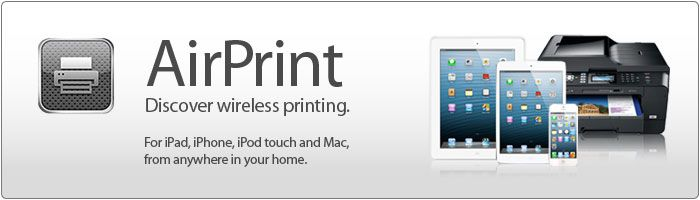
\includegraphics[scale=0.6]{airprint}
	\end{figure}

	\framebreak
	\begin{block}{Airprint}
		AirPrint é uma tecnologia da Apple que ajuda você a criar impressões de alta qualidade por meio do iPhone, iPad, Mac ou Apple Vision Pro
		sem precisar baixar ou instalar drivers. Os recursos do AirPrint incluem fácil localização, seleção automática de mídia e opções de 
		acabamento profissional.

		\begin{enumerate}
			\item Conecte a impressora à rede Wi-Fi.
			\item Certifique-se de que o iPhone, iPad, Mac ou Apple Vision Pro esteja conectado à mesma rede Wi-Fi da impressora.
			\item Para imprimir a partir de um app no dispositivo Apple, selecione a impressora na caixa de diálogo de impressão do app e, em seguida, imprima.
		\end{enumerate}
	\end{block}

	\framebreak
	\begin{block}{Bonjour}
		Os Serviços de Impressão do Bonjour para Windows permitem detectar e configurar impressoras compatíveis com o Bonjour a partir de um computador
		Windows através do Assistente de Impressora do Bonjour.
		O protocolo de rede do Bonjour envia e recebe pacotes de rede pela porta UDP 5353. O instalador do Bonjour irá configurar o firewall do Windows adequadamente
		durante a instalação nos sistemas compatíveis, mas se você tiver um outro firewall ativado, certifique-se de que a porta UDP 5353 está aberta para que 
		o Bonjour funcione corretamente.
	\end{block}

\end{frame}

\begin{frame}[allowframebreaks]{Evolução da Impressão}
	\begin{figure}
		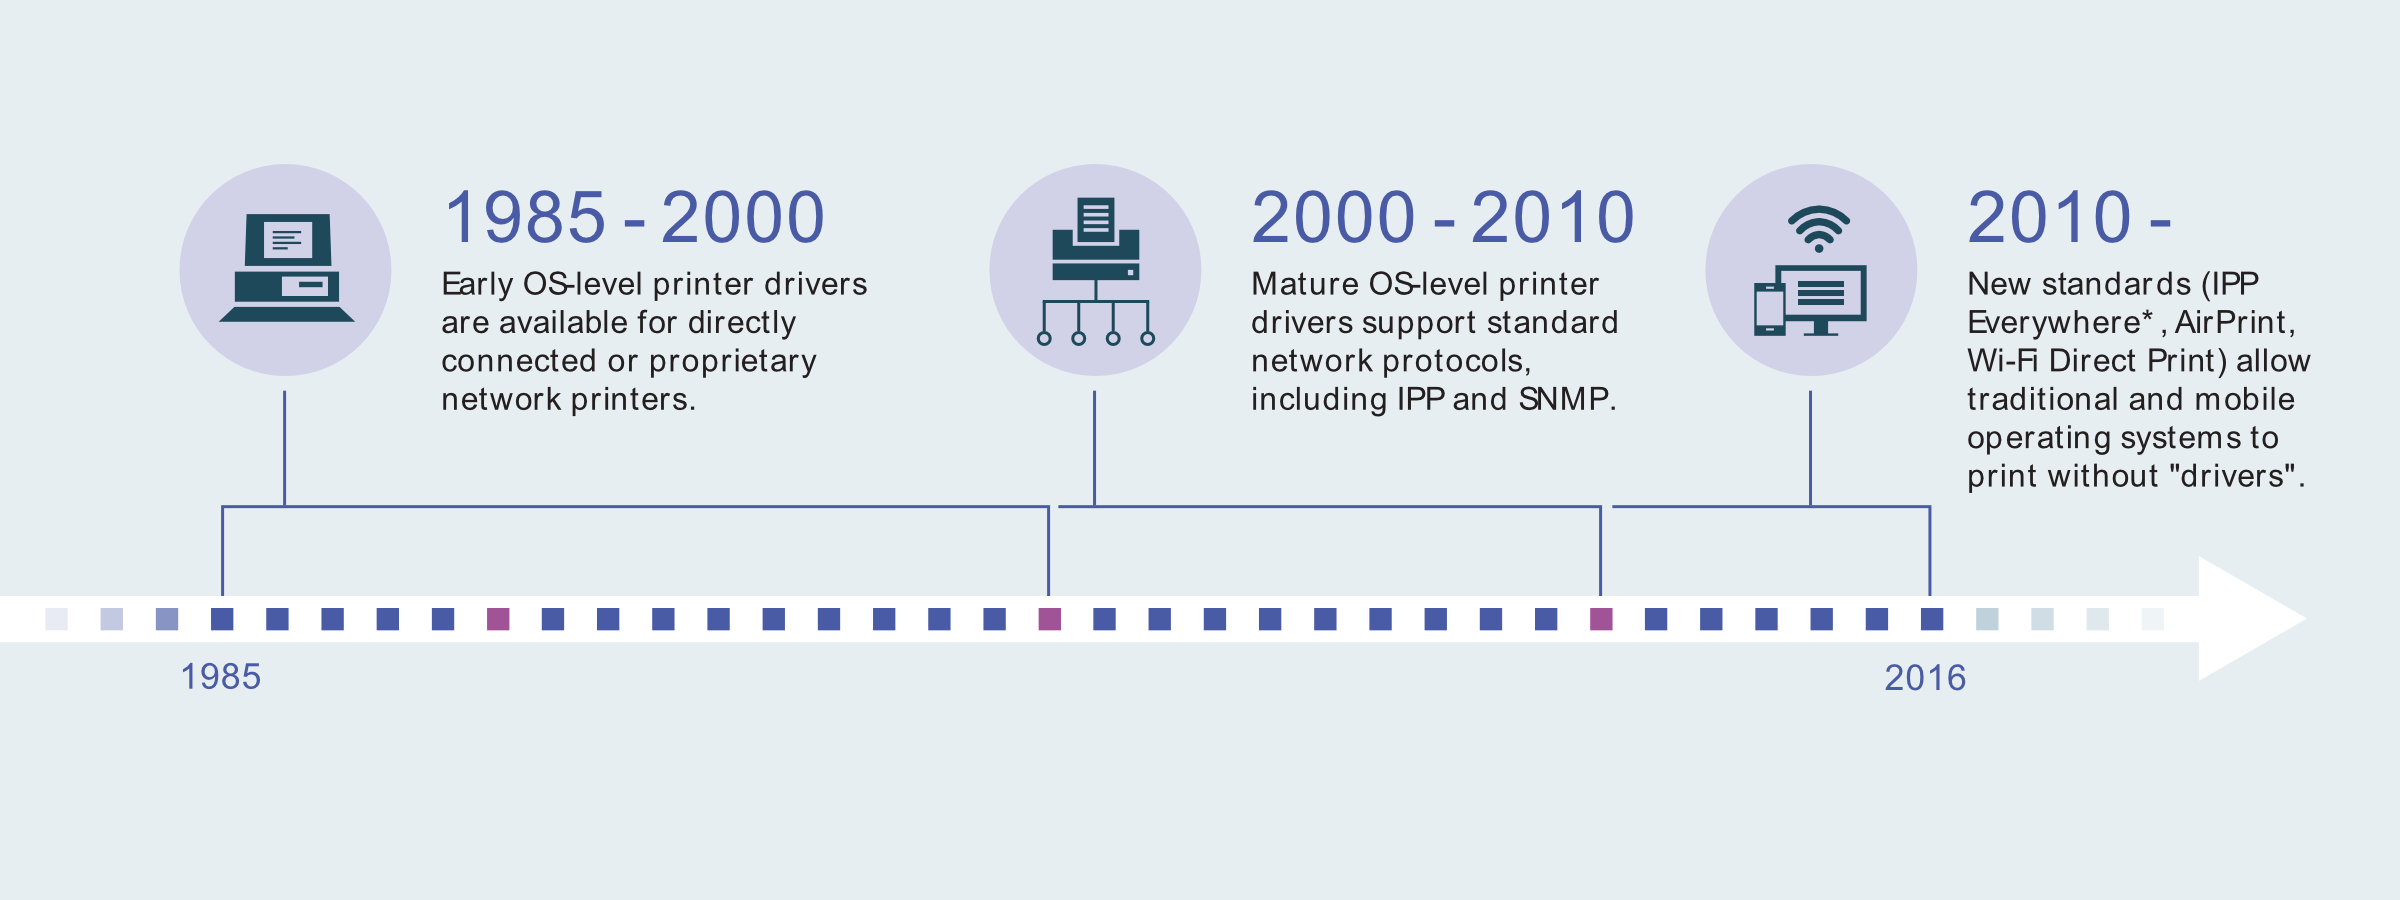
\includegraphics[scale=1]{timeline}
	\end{figure}
\framebreak
	\begin{figure}
		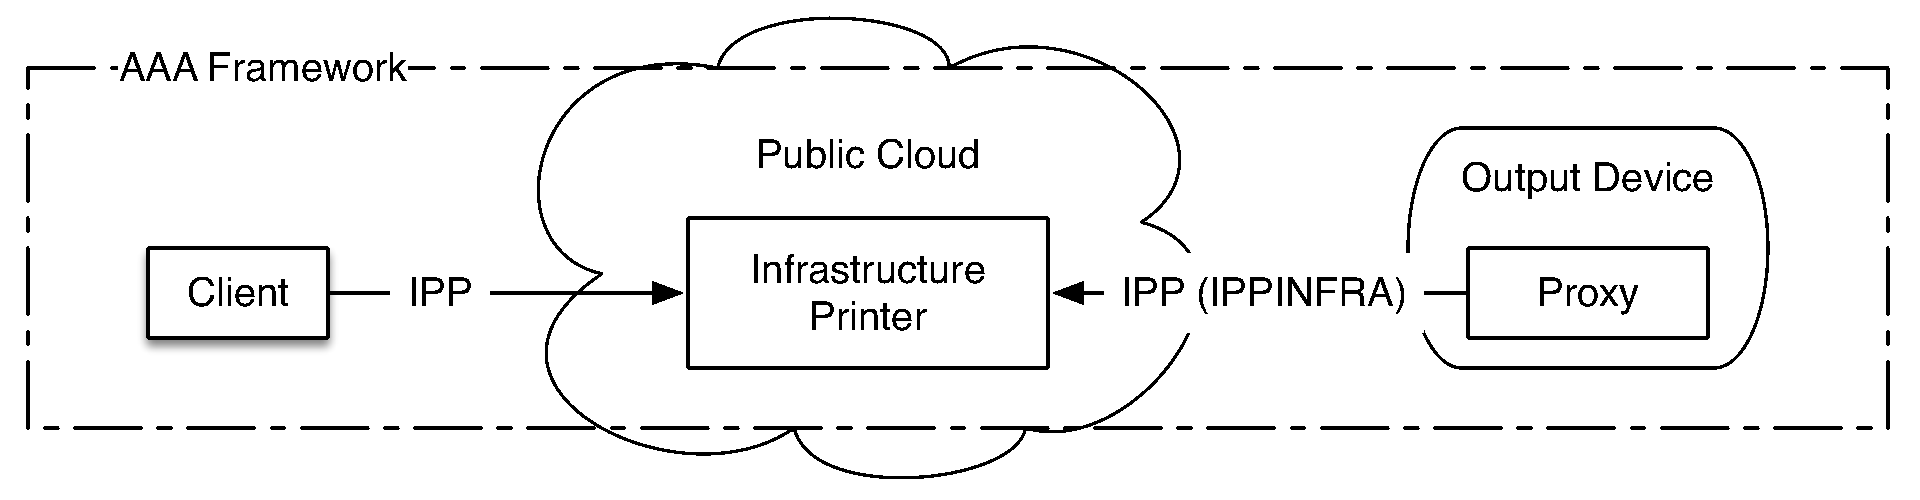
\includegraphics[scale=0.8]{cloud}
	\end{figure}
\end{frame}

\begin{frame}{Forks}
	\begin{figure}
		
\includegraphics[scale=0.7]{fork}
	\end{figure}
	
\end{frame}
\begin{frame}[allowframebreaks]{CUPS}
	O CUPS é um servidor de impressão, e como todo servidor, ele serve a um cliente que pode ser o computador do usuário, ou uma série de computadores 
	que precisam realizar uma impressão mas não possuem uma impressora física conectada a ele.

	Ele também pode trabalhar como um cliente, conectando-se ao computador ``servidor" e enviando o pedido de impressão, mesmo que não possua 
	os drivers da impressora que será utilizada, basta saber o ``endereço" da impressora no servidor.
	\framebreak

	O Common UNIX Printing System, ou CUPS, é a forma mais utilizada para gerir a impressão e os serviços de impressão. Este sistema de impressão disponível gratuitamente
    tornou-se o padrão para a impressão na maioria das distribuições Linux e utiliza o Protocolo de Impressão pela Internet (IPP) padrão
    para gerir a impressão em rede.

	O CUPS gere trabalhos e filas de impressão e oferece suporte a uma vasta gama de impressoras, desde as matriciais às laser, passando por muitos outros tipos.
    O CUPS também suporta a Descrição de Impressora PostScript (PPD) e a deteção automática de impressoras em rede, além de dispor de uma ferramenta simples de configuração
    e administração baseada na Web.

\end{frame}

\begin{frame}{CUPS compatibilidade}
	CUPS funciona/compatível com:
\begin{itemize}
	\item AirPrint$^{TM}$ and IPP Everywhere$^{TM}$ printers
	\item Network and local (USB) printers with Printer Applications 
	\item Network and local (USB) printers with (legacy) PPD-based printer drivers.
\end{itemize}	
\end{frame}

\begin{frame}{Instalação no Debian (máquina virtual)}
\begin{center}
	\texttt{sudo apt install cups -y}
\end{center}
\end{frame}

\begin{frame}{Interface web}
	\begin{figure}
		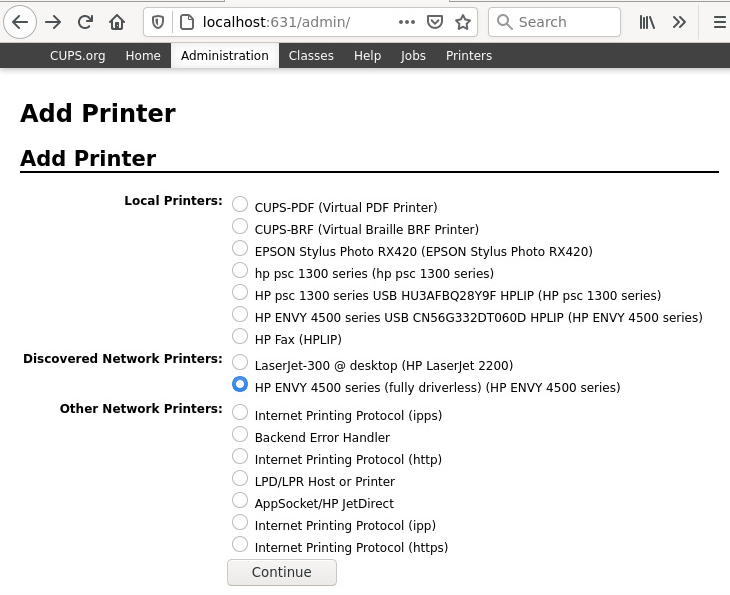
\includegraphics[scale=1]{cups-web}
	\end{figure}
\end{frame}

\begin{frame}{Gerenciamento de serviços}
		\begin{figure}
			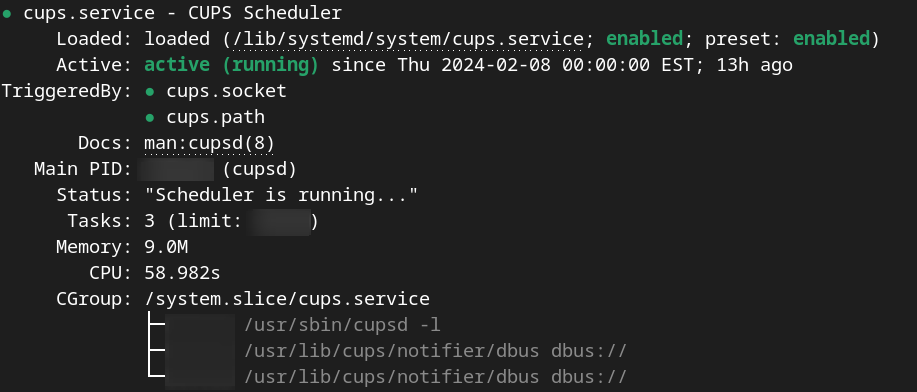
\includegraphics[scale=1]{System-Ctl-CUPS}
		\end{figure}
\end{frame}

\begin{frame}[allowframebreaks]{Referências Bibliográficas}
		\bibitem{noauthor_undated-xq}
	NTP.br. \url{https://ntp.br/conteudo/ntp/}. Acessado em: 6 de agosto de 2026.

		\bibitem{Cisco_System_Inc2022-gp}
		Cisco System, Inc. (2022). Identificar e Solucionar Problemas do Network Time Protocol (NTP). 26 de setembro de 2022.

		\bibitem{ibm}
		IBM. (2025). Tivoli Application Dependency Discovery Manager. \url{https://www.ibm.com/docs/pt-br/taddm/7.3.0?topic=problems-synchronization-server}. Acessado em: 6 de agosto de 2026.

		\bibitem{cisco}
		Cisco. (2025). Use as práticas recomendadas para o Network Time Protocol. \url{https://www.cisco.com/c/pt_br/support/docs/availability/high-availability/19643-ntpm.html}. Acessado em: 6 de agosto de 2026.

		\bibitem{suse}
		SUSE. (2026). Sincronizando o horário por meio de NTP/NTS. \url{https://documentation.suse.com/pt-br/sle-micro/6.1/html/Micro-ntp-time-synchronization/index.html}. Acessado em: 6 de agosto de 2026.

		\bibitem{Moreiras2021}
		Moreiras, Antonio Marcos. (2021). NTP e NTS de Forma Correta e Segura, Sincronismo de Tempo na Internet. Nic.br. \url{https://bibliotecadigital.acervo.nic.br/server/api/core/bitstreams/129d1169-25b5-49ce-b015-28ffadc440da/content}. Acessado em: 6 de agosto de 2026.
\end{frame}	
	
\end{document}
